\vspace{0.5cm}
Une fois que nous avons les données prêtes, nous pouvons procéder à l'entraînement.

\vspace{0.5cm}
\textbf{Les étapes:}

\begin{enumerate}
	\item Entraîner un modèle par classe : \textit{Poe} et \textit{Frost}
	\begin{itemize}
		\item N'oubliez pas les équations !
	\end{itemize}
	\item N'oubliez pas d'utiliser la propriété \textit{smoothing} (e.g. \textit{one-smoothin}). 
	\item Considérer si c'est nécessaire d'utiliser $A$ et $\pi$ ou $log(A)$ et $log(\pi)$.
	\item Afin d'appliquer les règles bayésiennes, calculez aussi les \textit{priors} \textbf{p(class=k)}
	\item Maintenant vous avez tout pour faire une prédiction.
	\item Écrire une fonction python pour calculer les \textit{posterior} (pour chaque classe) à partir d'un texte donnée comme \textit{input}.
	\item Prenez l'\textit{argmax} parmi les \textit{posterior} calcules pour obtenir las classe prédite.
	\item Faites des prédictions avec le corpus d'entraînement et le corpus de teste.
	\item Calculez la précision 
	\begin{itemize}
		\item lFALTA
	\end{itemize}
	\item F-Score et matrice de confusion.
	
\end{enumerate}

\begin{figure}[h]
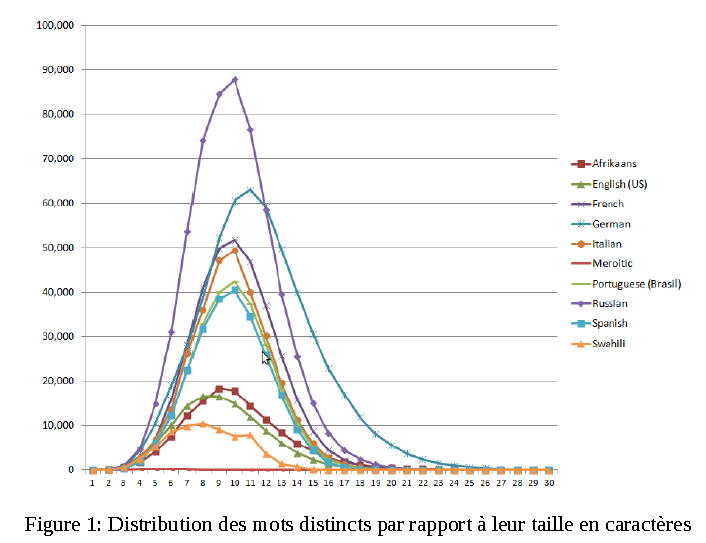
\includegraphics[width=0.6\textwidth]{../images/distrib.png}
\caption{Distribution des mots par rapport à leur taille en caractères dans
différentes langues\label{distrib}}
\end{figure}

L'axe des abscisses représente la taille d'un mot en caractères et
l'axe des ordonnées représente le nombre de mots uniques correspondant
à cette taille.

Pour préparer votre espace de travail sur votre notebook \textsc{Jupyter},
créez un dossier TD1 dans lequel vous enregistrerez votre code et
vos données.

Pous constituer un corpus, vous utiliserez les fichiers textes suivants
(choisissez plain text utf-8): 
\begin{itemize}
\item "Le discours de la méthode" (fr) \url{http://www.gutenberg.org/ebooks/13846}
%. Pour que les résultats soient plus significatifs, pensez à supprimer les premières phrases du fichier écrites en anglais.
\item "Ulysses" (en) \url{http://www.gutenberg.org/ebooks/4300} 
\end{itemize}
\newpage{}

\textbf{Les étapes :}
\begin{enumerate}
\item \textbf{lire} les textes 
\item \textbf{découper} en mots (ou tokeniser) 
\item \textbf{compter} le nombre de mots par taille de caractères 
\item \textbf{observer} les résultats chiffrés 
\item \textbf{représenter} cela sur une courbe 
\end{enumerate}
\textbf{Etape 1 : lire}

On ouvre le fichier en indiquant son chemin (\textit{path}), si vous
avez bien enregistré votre fichier au même endroit que votre code,
le nom du fichier suffit .

\textbf{Si ça ne marche pas c'est que} : 
\begin{itemize}
\item Tout n'est pas au bon endroit (\texttt{File not Found}), regardez
dans l'onglet \texttt{files} de \textsc{Jupyter} pour voir où vous
êtes. 
\item ou que on a un problème d'encoding (\texttt{charmap}), il faut ajouter
ecoding ='utf-8' dans le open : open("13846-0.txt", encoding ="utf-8") 
\end{itemize}
Nous allons commencer par le "Discours de la Méthode", si vous avez
conservé le nom d'origine il devrait s'appeler "13846-0.txt".

\begin{python} with open("13846-0.txt") as f: chaine = f.read()
\end{python}

Et on affiche un bout du texte pour vérifier que ça marche :

\begin{python} print(chaine{[}:100{]}) \end{python}

\textbf{Etape 2 : découper}

On va très simplement découper en mots avec la \textbf{méthode} \textit{split}
\begin{python} listemots = chaine.split()\#approximation des occurrences
print("Nombre de mots : %i" %len(liste_mots))
\end{python}

\textbf{Etape 3 : compter}

On va utiliser un \textbf{dictionnaire} (ou tableau associatif) où
l'on va stocker pour chaque longueur en caractères le nombre de mots
qu'on a rencontré. Le fonctionnement est le suivant: 
\begin{itemize}
\item pour chaque mot de la liste de mots, on calcule sa longueur 
\item on vérifie si on a déjà rencontré un mot de cette longueur: 
\begin{itemize}
\item Si c'est le premier mot pour cette longueur on crée une \textbf{clé}
pour cette longueur à laquelle on affecte la \textbf{valeur} 1 
\item Sinon, on \textbf{incrémente} de 1 la valeur existante 
\end{itemize}
\end{itemize}
\begin{python} diclongueurs = {} \#un dictionnaire vide

for mot in listemots: longueur = len(mot)\#la longueur du mot if longueur
not in diclongueurs: \#on a jamais vu cette longueur de mot diclongueurs{[}longueur{]}=1
\# else: \#on a vu cette longueur de mot diclongueurs{[}longueur{]}+=1

print(diclongueurs)\#pour avoir une vue de ce qu'on a fait

\end{python}

NB: si le processus ne vous semble pas clair, ajoutez au début de
la boucle \textit{for} deux lignes (avec l'indentation) pour suivre
le processus pas à pas :

\begin{python} print(diclongueurs) dd=input("Appuyez sur Enter pour
passer a la suite") \end{python}

\textbf{Etape 4: observer}

Un dictionnaire n'est pas une structure de données ordonnée, pour
vérifier que'on trouve des résultats proche de l'attendu, on va afficher
le nombre d'occurences enregistré dans \texttt{dic\_longueurs} pour
toutes les longueurs de 1 à 30 en utilisant \textbf{l'itérateur} \textit{range}.
Dans le \textit{print} on utilise du \textbf{formatage de chaînes
de caractères}\footnote{Voir par exemple \url{https://stackoverflow.com/questions/5082452/string-formatting-vs-format}}.

\begin{python} for toto in range(1, 31):\#de 1 à 30 (31 est exclu)
nbroccurences = diclongueurs{[}toto{]} print("%i : %i"%(toto, nbr_occurences))
\end{python}

Vous verrez que le code plante car on a des longueurs qui ne sont
pas dans le dictionnaire, on va donc améliorer le code de la façon
suivante:

\begin{python} for toto in range(30): if toto in diclongueurs: nbroccurences
= diclongueurs{[}toto{]} print("%i : %i"%(toto, nbr_occurences))
 else: nbroccurences = 0 print("%i : %i"%(toto, nbr_occurences))
\end{python}

\textbf{Etape 5 : représenter}

Et maintenant c'est magique, on va créer une courbe grâce à la librairie
\texttt{matplotlib}. On va importer cette librairie et la renommer
pour que ça soit plus court à écrire. Puis pour avoir les valeurs
à mettre sur la courbe on va lire les valeurs dans l'ordre croissant
pour les ranger dans une liste nommée \textit{liste\_effectifs}. Pyplot
prend entrée un \textbf{vecteur}, une liste de valeurs ordonées.

\begin{python} import matplotlib.pyplot as pyplot \#import avec alias

listeeffectifs = {[}{]} for toto in range(30): if toto in diclongueurs:\#on
a donc vu des mots de cette longueur listeeffectifs.append(diclongueurs{[}toto{]})
else:\#on en n'a pas vu de cette longueur, on ajoute donc un 0 listeeffectifs.append(0)
pyplot.plot(listeeffectifs)\#on "dessine" pyplot.show()\#"on affiche"

\end{python}

\begin{figure}
\centering{}
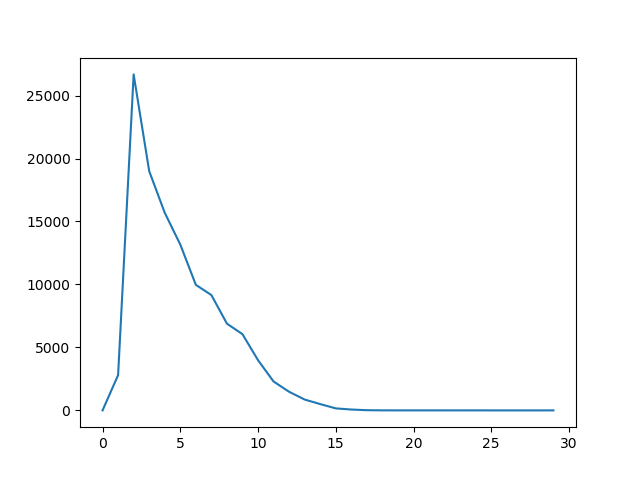
\includegraphics[width=0.5\textwidth]{../images/TD1_effectifs1.png}
\caption{"Discours de la Méthode" : nombre de mots par longueur (en abscisse),
en ordonnée l'effectif}
\end{figure}

Maintenant si on veut faire le même calcul pour l'autre texte on a
juste à changer le nom du fichier dans l'étape 1 et à relancer toutes
les cellules. Mais si on avait 100 textes à faire ça ne serait pas
très pratique. Nous allons donc voir dans l'exercice suivant comment
améliorer le code.
